\documentclass[journal]{IEEEtran}
\usepackage{blindtext}
\usepackage{graphicx}
\usepackage{amssymb}
\usepackage{tikz}
\usepackage{amsmath}
\usepackage{hyperref}
\usepackage[english]{babel}
\usepackage{graphicx}


\hyphenation{op-tical net-works semi-conduc-tor}


\begin{document}
\title{Graph Clustering Algorithms}
%
% author names and IEEE memberships
% note positions of commas and nonbreaking spaces ( ~ ) LaTeX will not break
% a structure at a ~ so this keeps an author's name from being broken across
% two lines.
% use \thanks{} to gain access to the first footnote area
% a separate \thanks must be used for each paragraph as LaTeX2e's \thanks
% was not built to handle multiple paragraphs
%

\author{Aleksandr~Salo, Rovshen~Nazarov
\thanks{Cho, Young-Rae is with the Department
of Electrical and Computer Engineering, Baylor University, Waco,
TX, 76706 USA}% <-this % stops a space
}

% note the % following the last \IEEEmembership and also \thanks - 
% these prevent an unwanted space from occurring between the last author name
% and the end of the author line. i.e., if you had this:
% 
% \author{....lastname \thanks{...} \thanks{...} }
%                     ^------------^------------^----Do not want these spaces!
%
% a space would be appended to the last name and could cause every name on that
% line to be shifted left slightly. This is one of those "LaTeX things". For
% instance, "\textbf{A} \textbf{B}" will typeset as "A B" not "AB". To get
% "AB" then you have to do: "\textbf{A}\textbf{B}"
% \thanks is no different in this regard, so shield the last } of each \thanks
% that ends a line with a % and do not let a space in before the next \thanks.
% Spaces after \IEEEmembership other than the last one are OK (and needed) as
% you are supposed to have spaces between the names. For what it is worth,
% this is a minor point as most people would not even notice if the said evil
% space somehow managed to creep in.



% The paper headers
\markboth{Baylor University, December~2014}%
{Graph Clustering Algorithms}
% The only time the second header will appear is for the odd numbered pages
% after the title page when using the twoside option.
% 
% *** Note that you probably will NOT want to include the author's ***
% *** name in the headers of peer review papers.                   ***
% You can use \ifCLASSOPTIONpeerreview for conditional compilation here if
% you desire.




% If you want to put a publisher's ID mark on the page you can do it like
% this:
%\IEEEpubid{0000--0000/00\$00.00~\copyright~2007 IEEE}
% Remember, if you use this you must call \IEEEpubidadjcol in the second
% column for its text to clear the IEEEpubid mark.



% use for special paper notices
%\IEEEspecialpapernotice{(Invited Paper)}




% make the title area
\maketitle


\begin{abstract}
%\boldmath
In this article we provide a brief overview of the few existing graph clustering algorithms that are commonly used in bioinformatics. Then we evaluate their performance and accuracy based on the sample protein-protein interaction network as an input and subgraphs representing potential protein complexes as an output. In particular we use  f-measure to evaluate the clustering results by comparing to protein complex data provided. For measuring the accuracy of the algorithms, we compute an f-score for each output cluster by selecting the maximum f-score to a protein complex, and average the f-scores of all output clusters. After evaluation we elaborate our own algorithm that tries to outperform the existing ones. 
\end{abstract}
% IEEEtran.cls defaults to using nonbold math in the Abstract.
% This preserves the distinction between vectors and scalars. However,
% if the journal you are submitting to favors bold math in the abstract,
% then you can use LaTeX's standard command \boldmath at the very start
% of the abstract to achieve this. Many IEEE journals frown on math
% in the abstract anyway.

% Note that keywords are not normally used for peerreview papers.
\begin{IEEEkeywords}
datamining, graphs, algorithms, bioinformatics
\end{IEEEkeywords}






% For peer review papers, you can put extra information on the cover
% page as needed:
% \ifCLASSOPTIONpeerreview
% \begin{center} \bfseries EDICS Category: 3-BBND \end{center}
% \fi
%
% For peerreview papers, this IEEEtran command inserts a page break and
% creates the second title. It will be ignored for other modes.
\IEEEpeerreviewmaketitle



\section{Introduction}
As a basis for the future comparison we implemented three different graph clustering algorithms:
\begin{enumerate}
	\item Common Neighbors Cut
	\item Common Neighbors Merge
	\item Seed Growth: Graph Entropy
\end{enumerate}

Text file describing all the edges of the graph was used as an input. Basic characteristics of the graph are the following:
\begin{figure}[h!]
\begin{center}
	\begin{tabular}{ | l | l |}
		\hline
		\multicolumn{2}{|c|}{Unweighted} \\ \hline
		\multicolumn{2}{|c|}{Disconnected} \\ \hline
		\multicolumn{2}{|c|}{Undirectedighted} \\ \hline
		Size ($|V|$)  & 2526  \\ \hline
		Edges ($|E|$) & 11450 \\ \hline
		Density & 0.00179  \\
		\hline
	\end{tabular}
\end{center}
\caption{Graph's Basic Characteristics}
\end{figure}
Let us now highlight the main ideas of implemented algorithms.

\subsection{Common Neighbors Cut}
This top-down hierarchical method generates non-overlapping clusters recursively dividing the initial graph using dissimilarity measure. \\
\textbf{The main idea is:} "Less common neighbors two vertices share, more dissimilar they are." [1]

Algorithm [3]:
\begin{enumerate}
	\item Iteratively eliminate the edge between the most dissimilar vertices
	based on a similarity function, until the graph is separated
	\item Recursively apply (1) into each subgraph
	\item Repeat (1) and (2) until all subgraphs reach a density threshold
\end{enumerate}

The main time consuming operation in the algorithm that repeatedly occurs is defining whether the graph is still connected (after removing the edge between two most dissimilar vertices) or not. Our implementation uses depth-first-search algorithm (which is very efficient) for deciding this question. 

\subsection{Common Neighbors Merge}
This algorithm is a mirrored brother of the previous one. Instead of recursively dividing the graph we initiate each node of the graph as a separate cluster. Then we merge most similar nodes until threshold value is violated. \\
\textbf{The main idea is:} "More common neighbors two vertices share, more similar they are." [2]

Algorithm [3]:
\begin{enumerate}
	\item Find the most similar vertices from different clusters based on a similarity
	function
	\item Merge the two clusters if the merged cluster reaches a density threshold
	\item Repeat (1) and (2) until no more clusters can be merged
\end{enumerate}

In order to avoid ~O($n^4$) calculation of the most similar nodes among all the clusters we initially calculate the table of distances for each pair of nodes and then look for the most relevant values.  

\subsection{Seed Growth: Graph Entropy}
This algorithm is a typical density-based algorithm which produces overlapping clusters via seed growth. \\
\textbf{The main idea is:} "Search for local optimization using a modularity (i.e. density) function." [4]

Algorithm [3]:
\begin{enumerate}
	\item Select a seed node among free vertices, and include all neighbors of the seed node into a seed cluster
	\item Iteratively remove a neighbor if removal decreases graph entropy
	\item Iteratively add a node on the outer boundary of a current cluster if addition decreases graph entropy
	\item Output the cluster with the minimal graph entropy
	\item Repeat (1), (2), (3), and (4) until no seed node remains
\end{enumerate}

Here entropy is a density measure (computable in ~O($|V|$) time) based on probabilities of having inner or outer links. [4] Seed selection is based on the vertex degree: the more degree is the more chances that the vertex would be a good seed.

Clearly, this algorithm runs very fast since it doesn't use recursion or nested loops among all the vertices.

\subsection{Implementation notes}
For all our algorithms we used the arbitrary chosen threshold value of 0.3. Also we tried to treat algorithms the same way and implement them using the same data structures (however authors of original papers used slightly different implementation). 

Our estimation is that the following tests should reflect the real measure of performance and accuracy.



\section{Performance and Accuracy Comparison}
For evaluation of accuracy we used the f-measure to evaluate the clustering results by comparing to protein complex data (ground truth), where f-measure is a harmonic mean of \textit{recall} and \textit{precision}:
\begin{center}
	f-measure = $\frac{2 * recall * precision}{recall + precision} $,\\	
\end{center} 
Recall (Sensitivity or True positive rate) = $\frac{|X \cap Y|}{|Y|}$\\
Precision (Positive predictive value) =  $\frac{|X \cap Y|}{|X|}$

Computing f-scores for the algorithm's accuracy is a three step process:\\
1. Compute all the f-measures for each resulting cluster.\\
2. Assign maximum f-measures to each cluster.\\
3. Take average f-measures as an f-score of the algorithm's accuracy. 

The process also described by the picture below:
\begin{figure}[h!]
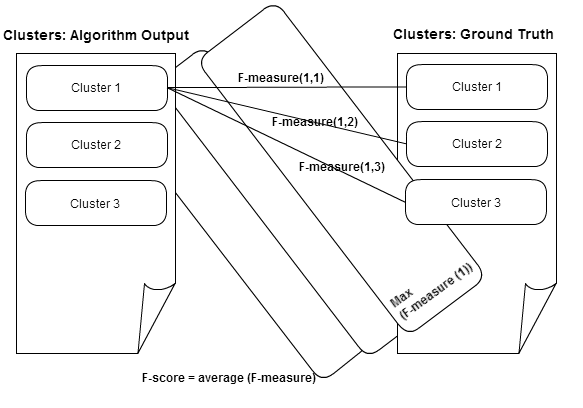
\includegraphics[width=3.4in,clip,keepaspectratio]{f-measure}
\caption{F-score process}
\end{figure}


Hereby accuracy could vary from 100\% (each of the resulting clusters are in the ground truth clusters) to 0\% (none of them fit).

\subsection{Accuracy and Runtime}

In this subsection we describe the experimental results that we obtained by running our implementation of three algorithms mentioned above. Accuracy is measured as described, runtime is simply an execution time in seconds. 
\begin{figure}[h!]
	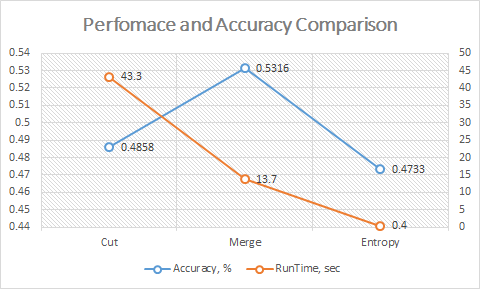
\includegraphics[width=3.4in,clip,keepaspectratio]{perfomance-comparison}
	\caption{Graph Clustering Algorithms: Accuracy and Runtime}
\end{figure}


Clearly, graph entropy algorithm is by far the fastest. However common neighbors merge perform slightly better results yet more efficient than common neighbors cut. 

\subsection{Distance measure}
While common neighbors merge algorithm produces good performance the accuracy could be varied with the use of different distant measures. Below we plot the accuracy for each of the following distance measures:
\begin{itemize}
	\item Jaccard Coefficient $S(x,y)=\dfrac{|N(x) \cap N(y)|}{|N(x) \cup N(y)|}$
	\item Maryland Bridge $S(x,y)=\dfrac{1}{2} (\dfrac{|N(x) \cap N(y)|}{|N(x)|} + \dfrac{|N(x) \cap N(y)|}{|N(y)|})$
	\item Dice $S(x,y)=\dfrac{2|N(x) \cap N(y)|}{|N(x)| + |N(y)|}$
	\item Simpson $S(x,y)=\dfrac{|N(x) \cap N(y)|}{min(|N(x)|, |N(y)|)}$
	\item Geometric $S(x,y)=\dfrac{|N(x) \cap N(y)|^2}{|N(x)| |N(y)|}$
\end{itemize}

\begin{figure}[h!]
	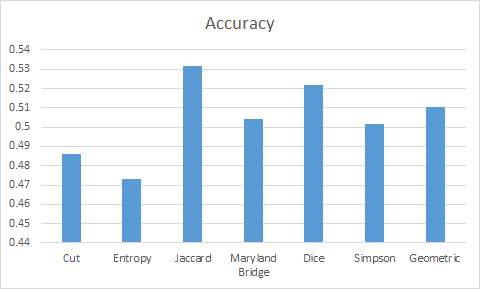
\includegraphics[width=3.4in,clip,keepaspectratio]{distance-measures}
	\caption{Algorithms' Accuracy}
	
\end{figure}


Clearly, for this specific dataset of protein-protein interaction Jaccard Coefficient measure works the best.

\subsection{Accuracy measure critique}
Although proposed accuracy measurement gives a good premise for comparing the algorithms it has somewhat serious lack: it biased toward the algorithms which produce the small number of clusters. Less cluster in the output - easier to fit them into ground truth. At the same time less clusters could mean a loss of opportunities with the real biological value. 

On the picture below we provide a plot with the number of clusters produced by different algorithms:
\begin{figure}[h!]
	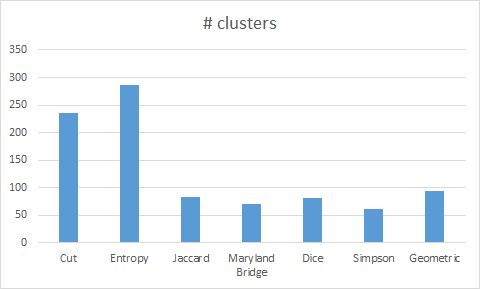
\includegraphics[width=3.4in,clip,keepaspectratio]{num-clusters}\
	\caption{Algorithms' number of clusters produced}	
\end{figure}
Common Neighbors Cut and Seed Growth by Entropy methods provide two-three times more clusters than the Common Neighbors Merge algorithms with different measures. This affects the accuracy significantly (strong negative correlation between the number of clusters produced and accuracy is visible from the plots), however the extra clusters might bear more useful and meaningful information. 

At the end of the day it is up to a scientist who uses the algorithm to decided which behavior is preferable due to the context of the problem.

\section{Rovshen}
gdfg\\
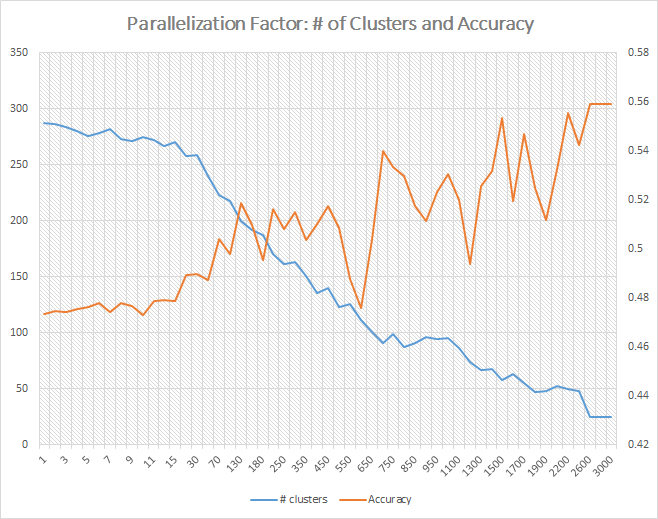
\includegraphics[width=3.4in,clip,keepaspectratio]{clusters-accuracy-parallel}
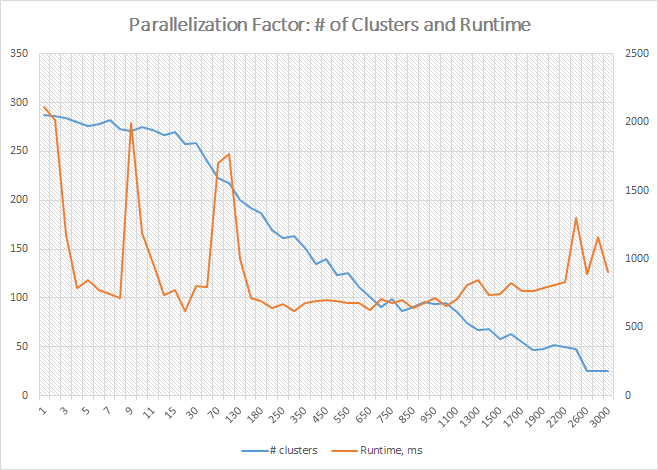
\includegraphics[width=3.4in,clip,keepaspectratio]{clusters-runtime-parallel}
% needed in second column of first page if using \IEEEpubid
%\IEEEpubidadjcol

% An example of a floating figure using the graphicx package.
% Note that \label must occur AFTER (or within) \caption.
% For figures, \caption should occur after the \includegraphics.
% Note that IEEEtran v1.7 and later has special internal code that
% is designed to preserve the operation of \label within \caption
% even when the captionsoff option is in effect. However, because
% of issues like this, it may be the safest practice to put all your
% \label just after \caption rather than within \caption{}.
%
% Reminder: the "draftcls" or "draftclsnofoot", not "draft", class
% option should be used if it is desired that the figures are to be
% displayed while in draft mode.
%
%\begin{figure}[!t]
%\centering
%\includegraphics[width=2.5in]{myfigure}
% where an .eps filename suffix will be assumed under latex, 
% and a .pdf suffix will be assumed for pdflatex; or what has been declared
% via \DeclareGraphicsExtensions.
%\caption{Simulation Results}
%\label{fig_sim}
%\end{figure}

% Note that IEEE typically puts floats only at the top, even when this
% results in a large percentage of a column being occupied by floats.


% An example of a double column floating figure using two subfigures.
% (The subfig.sty package must be loaded for this to work.)
% The subfigure \label commands are set within each subfloat command, the
% \label for the overall figure must come after \caption.
% \hfil must be used as a separator to get equal spacing.
% The subfigure.sty package works much the same way, except \subfigure is
% used instead of \subfloat.
%
%\begin{figure*}[!t]
%\centerline{\subfloat[Case I]\includegraphics[width=2.5in]{subfigcase1}%
%\label{fig_first_case}}
%\hfil
%\subfloat[Case II]{\includegraphics[width=2.5in]{subfigcase2}%
%\label{fig_second_case}}}
%\caption{Simulation results}
%\label{fig_sim}
%\end{figure*}
%
% Note that often IEEE papers with subfigures do not employ subfigure
% captions (using the optional argument to \subfloat), but instead will
% reference/describe all of them (a), (b), etc., within the main caption.


% An example of a floating table. Note that, for IEEE style tables, the 
% \caption command should come BEFORE the table. Table text will default to
% \footnotesize as IEEE normally uses this smaller font for tables.
% The \label must come after \caption as always.
%
%\begin{table}[!t]
%% increase table row spacing, adjust to taste
%\renewcommand{\arraystretch}{1.3}
% if using array.sty, it might be a good idea to tweak the value of
% \extrarowheight as needed to properly center the text within the cells
%\caption{An Example of a Table}
%\label{table_example}
%\centering
%% Some packages, such as MDW tools, offer better commands for making tables
%% than the plain LaTeX2e tabular which is used here.
%\begin{tabular}{|c||c|}
%\hline
%One & Two\\
%\hline
%Three & Four\\
%\hline
%\end{tabular}
%\end{table}


% Note that IEEE does not put floats in the very first column - or typically
% anywhere on the first page for that matter. Also, in-text middle ("here")
% positioning is not used. Most IEEE journals use top floats exclusively.
% Note that, LaTeX2e, unlike IEEE journals, places footnotes above bottom
% floats. This can be corrected via the \fnbelowfloat command of the
% stfloats package.



\section{Conclusion}
\blindtext





% if have a single appendix:
%\appendix[Proof of the Zonklar Equations]
% or
%\appendix  % for no appendix heading
% do not use \section anymore after \appendix, only \section*
% is possibly needed

% use appendices with more than one appendix
% then use \section to start each appendix
% you must declare a \section before using any
% \subsection or using \label (\appendices by itself
% starts a section numbered zero.)
%


\appendices
\section{Proof of the First Zonklar Equation}
Some text for the appendix.

% use section* for acknowledgement
\section*{Acknowledgment}

The $\Sigma$ authors would like to thank...


% Can use something like this to put references on a page
% by themselves when using endfloat and the captionsoff option.
\ifCLASSOPTIONcaptionsoff
  \newpage
\fi



% trigger a \newpage just before the given reference
% number - used to balance the columns on the last page
% adjust value as needed - may need to be readjusted if
% the document is modified later
%\IEEEtriggeratref{8}
% The "triggered" command can be changed if desired:
%\IEEEtriggercmd{\enlargethispage{-5in}}

% references section

% can use a bibliography generated by BibTeX as a .bbl file
% BibTeX documentation can be easily obtained at:
% http://www.ctan.org/tex-archive/biblio/bibtex/contrib/doc/
% The IEEEtran BibTeX style support page is at:
% http://www.michaelshell.org/tex/ieeetran/bibtex/
%\bibliographystyle{IEEEtran}
% argument is your BibTeX string definitions and bibliography database(s)
%\bibliography{IEEEabrv,../bib/paper}
%
% <OR> manually copy in the resultant .bbl file
% set second argument of \begin to the number of references
% (used to reserve space for the reference number labels box)
\begin{thebibliography}{1}
 
\bibitem{IEEEhowto:Radicchi}Radicchi, Filippo, Claudio Castellano, Federico Cecconi, Vittorio Loreto, and Domenico Parisi. “Defining and Identifying Communities in Networks.” Proceedings of the National Academy of Sciences of the United States of America 101, no. 9 (March 2, 2004): 2658–63. doi:10.1073/pnas.0400054101.

\bibitem{IEEEhowto:Brun}
Brun, Christine, Carl Herrmann, and Alain Guénoche. “Clustering Proteins from Interaction Networks for the Prediction of Cellular Functions.” BMC Bioinformatics 5, no. 1 (July 13, 2004): 95. doi:10.1186/1471-2105-5-95.

\bibitem{IEEEhowto:Cho} Cho, Young-Rae. "CSI 4352, Introduction to Data Mining." 10/16/2014 (n.d.): n. pag. Web. \url{http://web.ecs.baylor.edu/faculty/cho/4352/9_GraphMining.pdf}

\bibitem{IEEEhowto:Cho} Chiam, Tak C., and Young-Rae Cho. “Accuracy Improvement in Protein Complex Prediction from Protein Interaction Networks by Refining Cluster Overlaps.” Proteome Science 10, no. Suppl 1 (June 21, 2012): S3. doi:10.1186/1477-5956-10-S1-S3.


\end{thebibliography}

% biography section
% 
% If you have an EPS/PDF photo (graphicx package needed) extra braces are
% needed around the contents of the optional argument to biography to prevent
% the LaTeX parser from getting confused when it sees the complicated
% \includegraphics command within an optional argument. (You could create
% your own custom macro containing the \includegraphics command to make things
% simpler here.)
%\begin{biography}[{\includegraphics[width=1in,height=1.25in,clip,keepaspectratio]{mshell}}]{Michael Shell}
% or if you just want to reserve a space for a photo:

\begin{IEEEbiography}[{
\includegraphics[width=1in,height=1.25in,clip,keepaspectratio]{picture}}]{John Doe}
\blindtext
\end{IEEEbiography}

% You can push biographies down or up by placing
% a \vfill before or after them. The appropriate
% use of \vfill depends on what kind of text is
% on the last page and whether or not the columns
% are being equalized.

%\vfill

% Can be used to pull up biographies so that the bottom of the last one
% is flush with the other column.
%\enlargethispage{-5in}



% that's all folks
\end{document}


